%==============================================================================
% Figure: Holographic BEC Acoustic Black Hole
% Purpose: BEC acoustic black hole schematic with Hawking radiation analog
% Chapter: Ch25 - Holographic Experiments
% Type: Schematic
%==============================================================================

\begin{figure}[htbp]
  \centering
  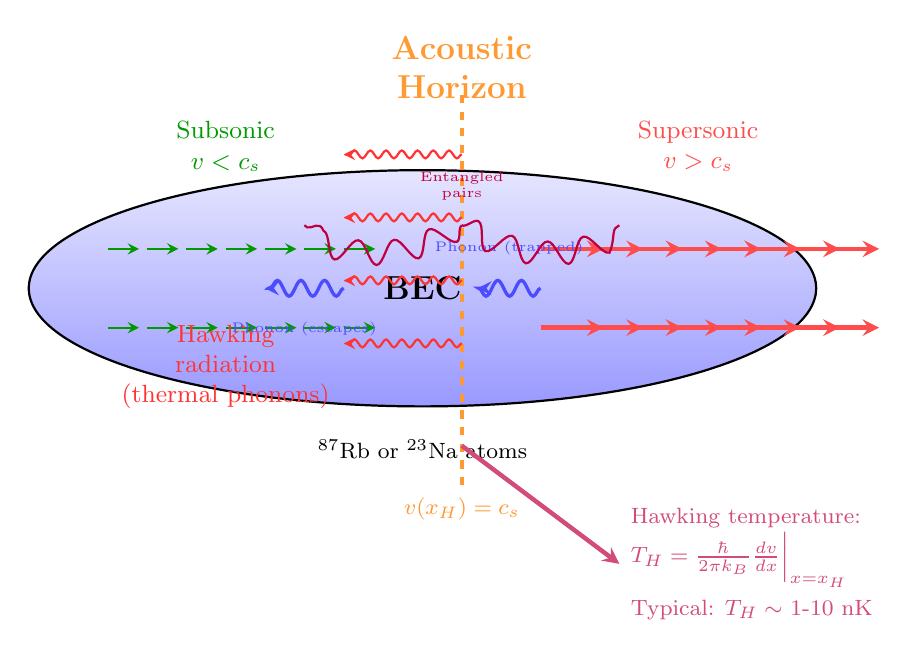
\begin{tikzpicture}[
    scale=1.0
  ]

    %========== BEC Cloud (elongated ellipse) ==========
    \shade[top color=blue!10, bottom color=blue!40, shading angle=0]
      (-6, 0) ellipse (5cm and 1.5cm);
    \draw[thick] (-6, 0) ellipse (5cm and 1.5cm);
    \node[font=\large\bfseries] at (-6, 0) {BEC};
    \node[font=\footnotesize, below] at (-6, -1.8) {$^{87}$Rb or $^{23}$Na atoms};

    %========== Flow Velocity Profile (arrows) ==========
    % Subsonic region (left)
    \foreach \x in {-10, -9.5, -9, -8.5, -8, -7.5, -7} {
      \draw[->, >=stealth, thick, green!60!black] (\x, 0.5) -- ({\x + 0.4}, 0.5);
      \draw[->, >=stealth, thick, green!60!black] (\x, -0.5) -- ({\x + 0.4}, -0.5);
    }
    \node[font=\small, text=green!60!black, align=center] at (-8.5, 1.8) {Subsonic\\$v < c_s$};

    % Supersonic region (right)
    \foreach \x in {-4.5, -4, -3.5, -3, -2.5, -2, -1.5, -1} {
      \draw[->, >=stealth, ultra thick, red!70] (\x, 0.5) -- ({\x + 0.8}, 0.5);
      \draw[->, >=stealth, ultra thick, red!70] (\x, -0.5) -- ({\x + 0.8}, -0.5);
    }
    \node[font=\small, text=red!70, align=center] at (-2.5, 1.8) {Supersonic\\$v > c_s$};

    %========== Acoustic Horizon (vertical line) ==========
    \draw[ultra thick, orange!80, dashed] (-5.5, -2.5) -- (-5.5, 2.5);
    \node[font=\large\bfseries, text=orange!80, align=center] at (-5.5, 2.8) {Acoustic\\Horizon};
    \node[font=\footnotesize, text=orange!80] at (-5.5, -2.8) {$v(x_H) = c_s$};

    %========== Sound Waves (phonons) ==========
    % Phonon inside horizon trying to escape (can't cross)
    \draw[->, >=stealth, very thick, blue!70, decorate, decoration={snake, amplitude=1mm, segment length=3mm}]
      (-4.5, 0) -- (-5.3, 0);
    \node[font=\tiny, text=blue!70, above] at (-4.9, 0.3) {Phonon (trapped)};

    % Phonon outside horizon escaping
    \draw[->, >=stealth, very thick, blue!70, decorate, decoration={snake, amplitude=1mm, segment length=3mm}]
      (-7, 0) -- (-8, 0);
    \node[font=\tiny, text=blue!70, below] at (-7.5, -0.3) {Phonon (escapes)};

    %========== Hawking Radiation (thermal phonons) ==========
    \foreach \i in {1, 2, 3, 4} {
      \pgfmathsetmacro\y{-1.5 + 0.8*\i}
      \draw[->, >=stealth, thick, red!80, decorate, decoration={snake, amplitude=0.5mm, segment length=2mm}]
        (-5.5, \y) -- (-7, \y);
    }
    \node[font=\small, text=red!80, align=center] at (-8.5, -1.0) {Hawking\\radiation\\(thermal phonons)};

    %========== Temperature Annotation ==========
    \draw[->, >=stealth, ultra thick, purple!70] (-5.5, -2.0) -- (-3.5, -3.5)
      node[right, align=left, font=\footnotesize] {
      Hawking temperature: \\
      $T_H = \frac{\hbar}{2\pi k_B} \frac{d v}{d x}\Big|_{x=x_H}$ \\
      \\
      Typical: $T_H \sim$ 1-10 nK
    };

    %========== Entanglement (Bell Pairs) ==========
    \draw[thick, purple, decorate, decoration={snake, amplitude=1.5mm, segment length=5mm}]
      (-5.5, 0.8) to[bend left=30] (-7.5, 0.8);
    \draw[thick, purple, decorate, decoration={snake, amplitude=1.5mm, segment length=5mm}]
      (-5.5, 0.8) to[bend right=30] (-3.5, 0.8);
    \node[font=\tiny, text=purple, align=center] at (-5.5, 1.3) {Entangled\\pairs};

  \end{tikzpicture}

  \vspace{0.5cm}

  %========== Velocity and Density Profiles ==========
  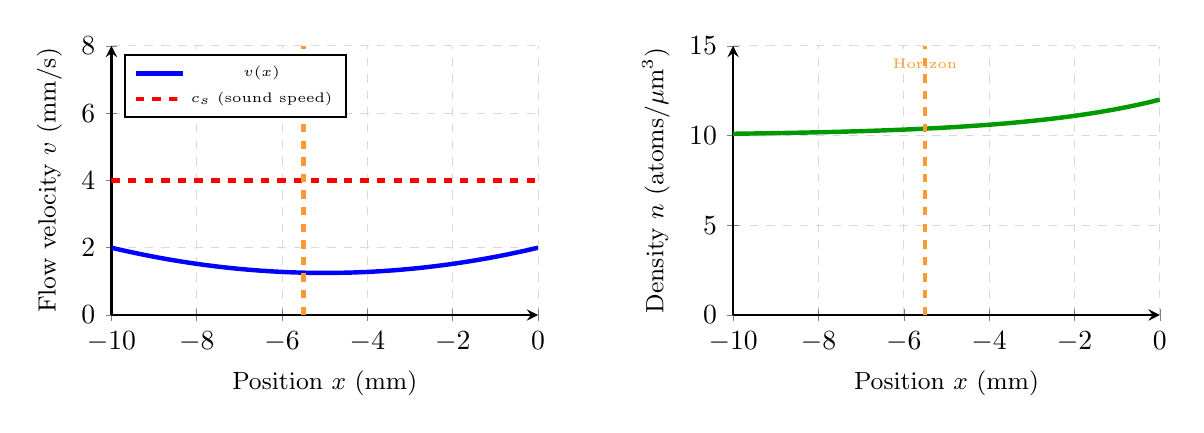
\begin{tikzpicture}[scale=1.0]
    %========== Velocity Profile ==========
    \begin{axis}[
      name=vel,
      width=7cm,
      height=5cm,
      xlabel={Position $x$ (mm)},
      ylabel={Flow velocity $v$ (mm/s)},
      xlabel style={font=\small},
      ylabel style={font=\small},
      xmin=-10, xmax=0,
      ymin=0, ymax=8,
      axis lines=left,
      grid=major,
      grid style={dashed, gray!30},
      samples=100,
      smooth,
      thick,
      legend pos=north west,
      legend style={font=\tiny}
    ]

      % Velocity profile (increases from left to right)
      \addplot[blue, ultra thick, domain=-10:0] {2 + 0.3*x + 0.03*x^2};
      \addlegendentry{$v(x)$}

      % Sound speed (constant)
      \addplot[red, ultra thick, dashed, domain=-10:0] {4};
      \addlegendentry{$c_s$ (sound speed)}

      % Mark horizon
      \draw[orange!80, ultra thick, dashed] (axis cs:-5.5, 0) -- (axis cs:-5.5, 8);
      \node[font=\tiny, text=orange!80] at (axis cs:-5.5, 7.5) {Horizon};

    \end{axis}

    %========== Density Profile ==========
    \begin{axis}[
      name=dens,
      at={(vel.right of south east)},
      anchor=left of south west,
      xshift=1cm,
      width=7cm,
      height=5cm,
      xlabel={Position $x$ (mm)},
      ylabel={Density $n$ (atoms/$\mu$m$^3$)},
      xlabel style={font=\small},
      ylabel style={font=\small},
      xmin=-10, xmax=0,
      ymin=0, ymax=15,
      axis lines=left,
      grid=major,
      grid style={dashed, gray!30},
      samples=100,
      smooth,
      thick
    ]

      % Density profile (decreases toward horizon)
      \addplot[green!60!black, ultra thick, domain=-10:0] {10 + 2*exp(0.3*x)};

      % Mark horizon
      \draw[orange!80, ultra thick, dashed] (axis cs:-5.5, 0) -- (axis cs:-5.5, 15);
      \node[font=\tiny, text=orange!80] at (axis cs:-5.5, 14) {Horizon};

    \end{axis}
  \end{tikzpicture}

  \vspace{0.5cm}

  %========== Explanation Boxes ==========
  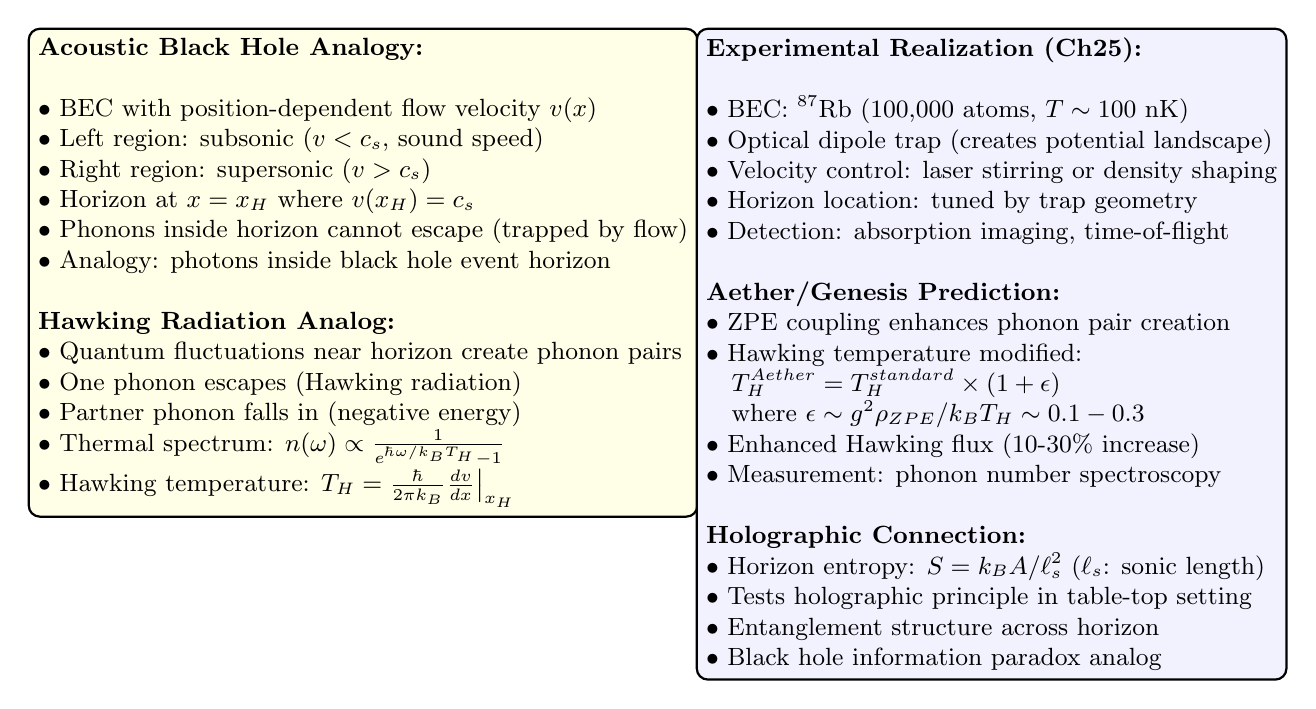
\begin{tikzpicture}
    \node[anchor=north west, align=left, font=\small, draw=black, fill=yellow!10, rounded corners, thick]
      at (0, 0) {
      \textbf{Acoustic Black Hole Analogy:} \\
      \\
      $\bullet$ BEC with position-dependent flow velocity $v(x)$ \\
      $\bullet$ Left region: subsonic ($v < c_s$, sound speed) \\
      $\bullet$ Right region: supersonic ($v > c_s$) \\
      $\bullet$ Horizon at $x = x_H$ where $v(x_H) = c_s$ \\
      $\bullet$ Phonons inside horizon cannot escape (trapped by flow) \\
      $\bullet$ Analogy: photons inside black hole event horizon \\
      \\
      \textbf{Hawking Radiation Analog:} \\
      $\bullet$ Quantum fluctuations near horizon create phonon pairs \\
      $\bullet$ One phonon escapes (Hawking radiation) \\
      $\bullet$ Partner phonon falls in (negative energy) \\
      $\bullet$ Thermal spectrum: $n(\omega) \propto \frac{1}{e^{\hbar\omega/k_B T_H} - 1}$ \\
      $\bullet$ Hawking temperature: $T_H = \frac{\hbar}{2\pi k_B}\frac{dv}{dx}\big|_{x_H}$
    };

    \node[anchor=north east, align=left, font=\small, draw=black, fill=blue!5, rounded corners, thick]
      at (16, 0) {
      \textbf{Experimental Realization (Ch25):} \\
      \\
      $\bullet$ BEC: $^{87}$Rb (100,000 atoms, $T \sim 100$ nK) \\
      $\bullet$ Optical dipole trap (creates potential landscape) \\
      $\bullet$ Velocity control: laser stirring or density shaping \\
      $\bullet$ Horizon location: tuned by trap geometry \\
      $\bullet$ Detection: absorption imaging, time-of-flight \\
      \\
      \textbf{Aether/Genesis Prediction:} \\
      $\bullet$ ZPE coupling enhances phonon pair creation \\
      $\bullet$ Hawking temperature modified: \\
      \quad $T_H^{\text{Aether}} = T_H^{\text{standard}} \times (1 + \epsilon)$ \\
      \quad where $\epsilon \sim g^2\rho_{\text{ZPE}} / k_B T_H \sim 0.1 - 0.3$ \\
      $\bullet$ Enhanced Hawking flux (10-30\% increase) \\
      $\bullet$ Measurement: phonon number spectroscopy \\
      \\
      \textbf{Holographic Connection:} \\
      $\bullet$ Horizon entropy: $S = k_B A / \ell_s^2$ ($\ell_s$: sonic length) \\
      $\bullet$ Tests holographic principle in table-top setting \\
      $\bullet$ Entanglement structure across horizon \\
      $\bullet$ Black hole information paradox analog
    };
  \end{tikzpicture}

  \caption{Acoustic black hole in a Bose-Einstein Condensate (BEC) as an analog system for testing
    Hawking radiation and holographic principles. The BEC cloud (blue ellipse, $^{87}$Rb or $^{23}$Na
    atoms) has a position-dependent flow velocity $v(x)$ (arrows): subsonic on the left (green,
    $v < c_s$) and supersonic on the right (red, $v > c_s$), where $c_s$ is the sound speed. At
    the acoustic horizon (orange dashed line, $x = x_H$), the flow velocity equals the sound speed:
    $v(x_H) = c_s$. Phonons (sound waves) inside the horizon (blue wavy arrows) cannot escape,
    analogous to photons trapped inside a black hole's event horizon. Quantum fluctuations near
    the horizon create entangled phonon pairs (purple wavy lines): one phonon escapes as Hawking
    radiation (red wavy arrows, thermal spectrum), while the partner falls in with negative energy.
    The Hawking temperature is $T_H = (\hbar/2\pi k_B)(dv/dx)|_{x_H}$, typically 1-10 nK. The
    Aether framework predicts that ZPE coupling enhances phonon pair creation, increasing the
    Hawking flux by 10-30\% ($\epsilon \sim 0.1$-$0.3$). Experimental protocols (Ch25) use BEC
    with $\sim 10^5$ atoms at 100 nK in optical dipole traps, with velocity controlled by laser
    stirring. The lower panels show velocity profile $v(x)$ (blue) crossing sound speed $c_s$ (red
    dashed) at the horizon, and density profile $n(x)$ (green). This table-top setup tests the
    holographic principle (horizon entropy $S \propto A$) and black hole physics, with Aether/Genesis
    frameworks predicting measurable enhancements in Hawking radiation.}
  \label{fig:holographic-bec}
\end{figure}
